% add style folder to path
\makeatletter
\def\input@path{{../style/}}
\makeatother

\documentclass[t, aspectratio=169, english, table]{tudelft-beamer}

\usepackage{datetime2}

% change the date format to "Month Year"
\makeatletter
\newcommand{\monthyeardate}{%
  \DTMenglishmonthname{\@dtm@month}, \@dtm@year
}
\makeatother

% figures and graphics
\usepackage{float}
\usepackage{graphicx}
\usepackage{ifthen}

% captions
\usepackage[labelfont=bf,justification=centering,footnotesize]{caption} 

% algrorithms
\usepackage{algorithm}
\usepackage{algpseudocode}
\usepackage{algorithmicx}

% section specific compilation
\includeonlyframes{%
  title,%
  opening,%
  toc,%
  questions,%
  background,%
  literature,%
  results,%
  outlook%
}

% extra colors
\definecolor{chapter}{HTML}{945357} % Deep Red

\addbibresource[type=file, glob, datatype=bibtex, location=local]{../bibliography.bib}

% redefine image path
\graphicspath{{../images}{../figures}}

% main title
\title[]{Sharpened CG Iteration Bound for Schwarz-preconditioned High-contrast Heterogeneous Scalar Elliptic PDEs}
\subtitle{Going Beyond Condition Number}
\author[]{P.~Soliman\inst{1}}

% define a graphic to be shown next to the title
\titlegraphic{\includegraphics[width=0.4\paperwidth]{two_cluster_respoly.png}}

\institute[University]{
  \strut\llap{\inst{1}\,}Delft University of Technology
}
\date[EEMCS-DIAM-NA MSc. Thesis \monthyeardate]{EEMCS-DIAM Numerical Analysis MSc. Thesis Presentation, \monthyeardate}

% command for including images
\newcommand{\absimage}[4][0.5,0.5]{%
	\begin{textblock}{#3}%width
		[#1]% alignment anchor within image (centered by default)
		(#2)% position on the page (origin is top left)
		\includegraphics[width=#3\paperwidth]{#4}%
\end{textblock}}

\begin{document}

\titleframe

\begin{frame}[label=opening]{Opening}
    \frametitle{Opening}
    \framesubtitle{Motivation}
        \begin{itemize}
            \item<1-> Opening question: "What do X, Y, Z have in common?". (Show X, Y and Z with single picture slides and make sure to give short descriptions. Go quickly through the single-picture slides.)
            \item<2-> Answer: "They can all be modelled by a..." high-contrast diffusion problem for $u, u_D \in H^1(\Omega)$, $f\in L^2(\Omega)$ and $\mathcal{C}\in L^{\infty}(\Omega)$
                  \begin{equation*}
                      \begin{aligned}
                          -\nabla\cdot\left(\mathcal{C}\nabla u\right) & = f \quad \text{in } \Omega           \\
                          u                                            & = u_D \quad \text{on } \partial\Omega
                      \end{aligned}
                  \end{equation*}
            \item<3-> Understanding the problem: We need to find $u \in H^1(\Omega)$ such that the above equation holds.
            \item<4-> Briefly explain why discretization is necessary for PDEs, for non-experts.
            \item<5-> FEM discretization $\Omega\rightarrow\mathcal{T}$, $\nabla \rightarrow A$, $u\rightarrow\mathbf{u}$, $f\rightarrow\mathbf{b}$
            \item<6-> Linear system of equations $A\mathbf{u}=\mathbf{b}$
            \item<7-> We can compute approximations $\mathbf{u}_1, \mathbf{u}_2, \ldots$ efficiently using the CG method.
            \item<8-> Main R.Q.: "How can we improve existing estimates on the total number of necessary CG iterations?"
        \end{itemize}
\end{frame}

\begin{frame}[label=toc]{Structure}
    \frametitle{Structure}
    \begin{itemize}
        \item CG method: under the hood
        \item Classical iteration bound
        \item Influence of eigenvalue distribution
        \item High-contrast coefficients: split eigenspectrum
        \item Two-cluster bound
        \item Multi-cluster bound
        \item Partitioning
        \item Results on sharpness
        \item Practical estimation of new bounds
    \end{itemize}
\end{frame}

\begin{comment}
Level 1: Discretisation & intro CG
- FEM discretization $\Omega\rightarrow\mathcal{T}$, $\nabla \rightarrow A$, $u\rightarrow\mathbf{u}$, $f\rightarrow\mathbf{b}$
- Linear system of equations $A\mathbf{u}=\mathbf{b}$
- CG takes in initial guess $\mathbf{u}_0$ and provides updated solution $\mathbf{u}_k$ after $k$ iterations.
- Classical bound given relative error tolerance $\epsilon_m = \frac{\|\mathbf{e}_m\|_A}{\|\mathbf{e}_0\|_A} \leq \epsilon$ is
$\epsilon_m \leq 2\left(\frac{\sqrt{\kappa} - 1}{\sqrt{\kappa} + 1}\right)^{m} \longrightarrow m \leq \left\lfloor\frac{\sqrt{\kappa}}{2}\ln\left(\frac{2}{\epsilon}\right) + 1\right\rfloor = m_1(\kappa)$
- However $m_1$ can be too pessimistic for high-contrast problems. That is, $m \ll m_1$
- Restate R.Q.: "How do we improve/sharpen the classical bound $m_1$ for model problem?"
Level 2: CG convergence in detail
- Spectrum $\sigma(A) = \{\lambda_1, \ldots, \lambda_n\}$ and $\kappa(A) = \frac{\lambda_{\max}}{\lambda_{\min}}$
- CG solution given as $\mathbf{u}_m = \mathbf{u}_0 + q(A)\mathbf{r}_0$, with polynomial $q$ being the \textit{solution polynomial}.
- CG residual polynomial $r(\lambda) = 1 - \lambda q(\lambda)$
- Error expression $\epsilon_m = \frac{\|\mathbf{e}_m\|_A}{\|\mathbf{e}_0\|_A} < \min_{r \in \mathcal{P}_{m-1}, r(0) = 1} \max_{\lambda \in \sigma(A)} |r(\lambda)|$
- Animation: cg_residual_poly
- Loop through different randomized, clustered spectra, showing r_m for each.
- Show best and worst case scenario's for CG convergence
- Restate R.Q.: "How can we construct an CG iteration bound that accounts for the influence of the eigenvalue distribution?"
Level 3: Preconditioning
- Why do we want to account for eigenvalue distribution? (practical motivation)
- High-contrast $C$ leads to spectral gap and $\kappa(A)\gg1$
- Preconditioning: transform $A\mathbf{u}=\mathbf{b}$ into $M^{-1}A\mathbf{u}=M^{-1}\mathbf{b}$, with preconditioner $M$. This leads to a reduced spectral gap and lower conditioner number. Then, apply CG as usual (now called Preconditioned CG or PCG)
- Show Filipe & Alexander's Research: they used three kinds of preconditioners $M_1, M_2, M_3$ and all had similar conditioner numbers and thereby similar upper bounds for their iteration number, $m_1(\kappa)$.
- However, on a sample problem PCG with $M_1,M_2$ needed significantly less iterations than PCG with $M_3$.
- Restate R.Q.: "How can we construct a CG iteration bound that can distinguish between different preconditioners with similar conditioner numbers?"
Level 4: First steps towards a sharpened bound
- Recap: $\epsilon_m < \min_{r \in \mathcal{P}_{m-1}, r(0) = 1} \max_{\lambda \in \sigma(A)} |r(\lambda)| \leq \epsilon$
- Head-on strategy for a bound: try to find an $m^{\text{th}}$-order polynomial that satisfies the min-max problem.
- Classical bound invokes: optimal Chebyshev polynomial $r(\lambda) = \hat{C}_m$, under the assumption of a uniform interval of eigenvalues $\sigma(A) = [\lambda_{\min}, \lambda_{\max}]$ (inaccurate!).
- Simplest non-trivial case (one spectral gap): two disjoint clusters
- Axelsson, assume two uniform intervals and invoke $r(\lambda) = \hat{C}_{p}\hat{C}_{p-m}$
- Resulting two-cluster bound $m_2(\kappa, \kappa_l, \kappa_r)=\left\lfloor\frac{\sqrt{\kappa_r}}{2} \ln (2 / \epsilon)+\left(1+\frac{\sqrt{\kappa_r}}{2} \ln \left(\frac{4\kappa}{\kappa_l}\right)\right) p\right\rfloor$
- Restate R.Q.: "How can we construct an CG iteration bound that accounts for the influence of the eigenvalue distribution for general spectra?"
Level 5: Generalization to multiple clusters & partitioning
- Depending on coefficient function and preconditioned systems we can have any number of clusters.
- Extend Axelsson idea: $r(\lambda) = \hat{C}^{(1)}_{p_1}\hat{C}^{(2)}_{p_2}\ldots\hat{C}^{(k)}_{p_k} = \prod_{i=1}^{k} \hat{C}^{(i)}_{p_i}$
- Multi-cluster bound: $p_i \leq \left\lceil\log_{f_i}{\frac{\epsilon}{2}} + \sum_{j=1}^{i-1} p_j\log_{f_i}\left(\frac{\zeta^{(j)}_2}{\zeta^{(i,j)}_1}\right)\right\rceil$ and $m_{N_{\text{cluster}}} = \sum_{i=1}^{N_{\text{cluster}}} p_i$, depends on the extremal eigenvalues of \textit{each cluster}
- We need a way of partitioning a given spectrum $\sigma(A)$ into $N_{\text{cluster}}$ clusters.
- Idea: simple, we split at the largest (relative) gap between subsequent eigenvalues, check if the two resulting clusters would give a sharper bound than just one uniform cluster, that is $m_2(\kappa, \kappa_l, \kappa_r) < m_1(\kappa)$. If so, we split the clusters and repeat the process for each created cluster. If not, we stop partitioning. In the process we keep track of all the extremal eigenvalues. After partitioning, we calculate $m_{N_{\text{cluster}}}$.
- Animation: cluster_partitioning, visualize above partitioning and subsequent calculation $m_{N_{\text{cluster}}}$.
- Restate R.Q.: "How much sharper is $m_{N_{\text{cluster}}}$ compared to $m_1(\kappa)$ for our model problem?"
Level 6: Results on sharpness
- We implement the model problem with the two coefficient functions that Filipe and Alexander used and solve them using PCG with preconditioners $M_1, M_2, M_3$.
- First experiment: For each $\sigma(M_i^{-1}A)$, we compute $m_{N_{\text{cluster}}}$ and $m_1(\kappa)$ for comparison. As well as, $m_{N_{\text{tail-cluster}}}$, a variant of $m_{N_{\text{cluster}}}$ that can take in clusters as well as individual eigenvalues.
- Results: the new bounds are incredibly sharp as they are anywhere from 2 to 4 times as big as $m$. For comparison, $m_1$ is anywhere from 100 to 1000 times bigger than $m$, where the difference increases for spectra with larger spectral gaps
- Restate R.Q.: "How can we compute $m_{N_{\text{cluster}}}$ for our model problem in practice?"
Level 7: Practical estimation of new bounds
- Problem: computing $m_{N_{\text{cluster}}}$ requires a good estimate of $\sigma(M_i^{-1}A)$.
- Luckily, PCG gives us exactly that, every iteration it produces a set of so-called Ritz values that is `close' to the true eigenvalue distribution. In particular, at the $k^{\text{th}}$ iteration, we get a set of $k$ Ritz values that we can use as an approximation of the full spectrum $\sigma(M_i^{-1}A)$.
- Second experiment, we use the Ritz values from the PCG iterations to compute $m_{N_{\text{cluster}}}$ and $m_1(\kappa)$ for our model problem and observe how good of an upper bound for $m$ we can obtain within the first 300 iterations.
- Results: For PCG with preconditioners $M_1, M_2$ (fast converging) $m_{N_{\text{cluster}}}$ gives sharp upper bounds for $m$ in all cases. However, for PCG with $M_3$ (slow converging) $m_{N_{\text{cluster}}}$ underestimates $m$ in some cases. This is because the Ritz values do not yet capture the full spectrum well enough within 300 iterations.
- Animation: ritz_value_migration
Level 8: Conclusion
- The main goal of this thesis was to sharpen the CG iteration bound for high-contrast heterogeneous scalar-elliptic problems beyond the classical condition number-based bound. The derived multi-cluster and tail-cluster bounds offer a more nuanced and accurate picture of convergence behavior than the classical condition number-based bound, able to distinguish between preconditioners effectively.
- Though the utility of these bounds for early estimation depends on the specific coefficient function and preconditioner used.
- Future work:
- Should focus on applying the new bounds to a wider range of problems, including those with more complex high-contrast coefficients, finer mesh discretizations, different preconditioners, and other types of PDEs.
- research into the \textit{a priori}  estimation of the key spectral characteristics ($\kappa_l, \kappa_r, s$) is crucial to circumvent the dependency of the new bounds on the slowly converging Ritz values
- Closer: "Today we learned to not judge a preconditioner by its conditioner number. Instead, we learned to look at the richness contained within the preconditioned spectrum... today, we truly went \textit{beyond condition number}."
\end{comment}

\chapter{Research questions}\label{ch:questions}\newpage
% \todo{Restate main research question – Clearly defined again.}\newline
% How can we sharpen the CG iteration bound for Schwarz preconditioned heterogeneous elliptic problems beyond the classical condition number based bound?
% \todo{Subsidiary questions – Justify why each one is important.}\newline
% \begin{enumerate}
%     \item How does the performance of the sharpened bounds vary with cluster width and eigengap?
%     \item Can we come up with more numbers like the condition number that can be used to estimate the eigenspectrum?
%     \item How do the improved bounds compare with existing bounds in the literature?
%     \item How do the improved bounds perform in the context of high-contrast Darcy problems?
%     \item How to estimate eigenspectrum beyond the condition number?
% \end{enumerate}

% \todo{Connection to literature gaps – Explain why your questions matter.}\newline
% \begin{enumerate}
%     \item Current work focuses on how to choose between several Schwarz preconditioners for the Darcy problem. The condition number alone does not help to a priori distinguish between these preconditioners. For instance In \cite{ams_coarse_space_comp_study_Alves2024} the AMS and GDSW preconditioners perform extraordinarily well compared to the RGDSW preconditioner. However, all three preconditioned systems share similar condition number. The only difference is in their spectral gap and cluster width. This motivates the need for a new number that can help distinguish between these preconditioners.
%     \item Application of sharpened bounds to distinguish between the performance of Schwarz-like preconditioners
%     \item Focus on application of the improved bounds to the Darcy problem in the context of Schwarz like preconditioners
% \end{enumerate}

% \todo{Expected challenges – Possible difficulties in answering them.}\newline
% One of the biggest challenges in sharpening the CG iteration bound lies in the quantitative estimation of the preconditioned system's spectrum. The literature on condition number estimation for Schwarz preconditioners is vast. For instance, in the simple cases of the additive Schwarz preconditioner with either a \cref{ASM_coarse_space:nicolaides} or \cref{ASM_coarse_space:local_eigenfunctions} an a priori estimate for the condition number is given by \cref{eq:two_level_ASM_condition_number} in combination with either \cref{eq:c0_nicolaides} or \cref{eq:c0_local_eigenfunctions}, respectively. The same can be said for the MsFEM and ACMS preconditioners. However, the literature lacks a quantitative estimate for the spectrum of the preconditioned system. This is crucial for sharpening the CG iteration bound. The lack of such an estimate is the main challenge in this work.

The main research question in this work is as follows:
\begin{researchq} \label{rq:main}
    \par
    How can we sharpen the CG iteration bound for Schwarz-preconditioned high-contrast heterogeneous elliptic problems beyond the classical condition number-based bound?
\end{researchq}
For instance, in \cite{ams_coarse_space_comp_study_Alves2024}, the AMS and GDSW preconditioners significantly outperform the RGDSW preconditioner, despite all three having similar condition numbers. The key differences appear in their spectral gap and cluster width, highlighting the need for additional spectral characteristics to refine existing bounds.

\begin{subsidiaryq} \label{rq:subsidiaries}
    To answer the main research question, we address the following subsidiary questions:
    \setlength\itemindent{1in}
    \begin{enumerate}[label=\textbf{Q\arabic*}, ref=Q\arabic*, leftmargin=1cm]
        \item\label{rq:subsidiary:measures} Which numerical measures, like the condition number, can we define to estimate the distribution of eigenvalues in the eigenspectrum in the case of high-contrast heterogeneous problems?
        \item\label{rq:subsidiary:estimation} How can we estimate any of the numerical measures defined in \ref{rq:subsidiary:measures} for the eigenspectrum in the particular case of a model Darcy problem?
        \item\label{rq:subsidiary:heuristic} Given a certain eigenspectrum, how can we sharpen the CG iteration bound?
        \item\label{rq:subsidiary:performance} How does the sharpened bound from \ref{rq:subsidiary:heuristic} perform for an unpreconditioned Darcy problem in comparison with the classical bound in \cref{eq:cg_convergence_rate}?
        \item\label{rq:subsidiary:dependance} How does the performance described in \ref{rq:subsidiary:performance} of a sharpened bound vary with the measures found in \ref{rq:subsidiary:measures}?
        \item\label{rq:subsidiary:preconditioners} Can we employ the sharpened bound to distinguish between the performance of Schwarz-like preconditioners? 
        \item\label{rq:subsidiary:formilization} Can we formalize a method to estimate the eigenspectrum beyond the condition number?
    \end{enumerate}
\end{subsidiaryq}

This research is important because current studies primarily focus on selecting between different Schwarz preconditioners for the Darcy problem, yet condition numbers fail to distinguish them effectively. The ability to differentiate preconditioners based on spectral properties would improve the selection process. Applying sharpened bounds could lead to better predictions of preconditioner performance and improved efficiency in solving high-contrast problems.

The main challenge lies in quantitatively estimating the spectrum of the preconditioned system. The literature provides a priori condition number estimates for various Schwarz preconditioners. For instance, in the simple cases of the additive Schwarz preconditioner with either a \cref{ASM_coarse_space:nicolaides} or \cref{ASM_coarse_space:local_eigenfunctions} an a priori estimate for the condition number is given by \cref{eq:two_level_ASM_condition_number} in combination with either \cref{eq:c0_nicolaides} or \cref{eq:c0_local_eigenfunctions}, respectively. The same can be said for the MsFEM and ACMS preconditioners. Despite this, there is no established method for estimating the full eigenspectrum. Without such an estimate, refining the CG iteration bound remains difficult. Overcoming this limitation is central to this work.

\begin{frame}[label=background]{Structure Background}
    \frametitle{Structure}
    \begin{itemize}
        \item Research Questions
        \item {\color{tud grapefruit}Background \& Literature}
        \item Preliminary Results
        \item Outlook
    \end{itemize}
\end{frame}

\footerinfootnotestrue
\begin{frame}[label=background,fragile]{Background: CG method}
    \frametitle{Background \& Literature}
    \framesubtitle{Conjugate gradient method}
    \begin{algorithm}[H]
        \begin{algorithmic}
            \State $\mathbf{r}_0 = \mathbf{b} - A\mathbf{u}_0$, $\mathbf{p}_0 = \mathbf{r}_0$, $\beta_0 = 0$
            \For{$j = 0, 1, 2, \dots, m$}
            \State $\alpha_j = (\mathbf{r}_j, \mathbf{r}_j) / (A \mathbf{p}_j, \mathbf{p}_j)$
            \State $\mathbf{u}_{j+1} = \mathbf{u}_j + \alpha_j \mathbf{p}_j$
            \State $\mathbf{r}_{j+1} = \mathbf{r}_j - \alpha_j A \mathbf{p}_j$
            \State $\beta_j = (\mathbf{r}_{j+1}, \mathbf{r}_{j+1}) / (\mathbf{r}_j, \mathbf{r}_j)$
            \State $\mathbf{p}_{j+1} = \mathbf{r}_{j+1} + \beta_j \mathbf{p}_j$
            \EndFor
        \end{algorithmic}
        \caption{Conjugate Gradient Method \cite{iter_method_saad}}
    \end{algorithm}
\end{frame}

\footerinfootnotesfalse
\begin{frame}[label=background,fragile]{Background: CG explained}
    \frametitle{Background \& Literature}
    \framesubtitle{Conjugate gradient method: residual polynomial}
    \begin{columns}[T,onlytextwidth]
        \begin{column}{.5\textwidth}
            \begin{itemize}
                \item<+-> Iterative, projection method onto a Krylov subspace $\mathcal{K}_m(A_0, \mathbf{r}_0)$ given by
                \begin{equation*}
                     \text{span}\{\mathbf{r}_0, A\mathbf{r}_0, A^2\mathbf{r}_0, \dots, A^{m-1}\mathbf{r}_0\}
                \end{equation*}
                \item<+-> Approximate solution can be expressed as
                \begin{equation*}
                    \mathbf{u}_m = \mathbf{u}_0 + \sum_{i=0}^{m-1} c_i A^i \mathbf{r}_0 = \mathbf{u}_0 + \alert<3>{q_{m-1}}(A)\mathbf{r}_0
                \end{equation*}
                \item<4> Minimize residual polynomial on eigenvalues of $A$
            \end{itemize}
        \end{column}
        \begin{column}{.5\textwidth}
            \only<3-4>{%
                \begin{figure}
                    \centering
                    \includegraphics[width=0.8\textwidth]{two_cluster_respoly.png}
                    \caption{Residual polynomial $r_m(\lambda) = 1 - \lambda \alert<3>{q_{m-1}}(\lambda)$}
                \end{figure}
            }
        \end{column}
    \end{columns}
\end{frame}

\begin{frame}[label=background,fragile]{CG convergence}
    \frametitle{Background \& Literature}
    \framesubtitle{Conjugate gradient method: convergence}
    \begin{itemize}
        \item<1-> Classical (condition number) convergence bound:
        \begin{theorem}
            The error of the $m^{\text{th}}$ iterate of the CG algorithm is bounded by
            \begin{equation*}
            ||\mathbf{e}_m|| \leq 2 \left(\frac{\sqrt{\kappa}-1}{\sqrt{\kappa} + 1}\right)^m ||\mathbf{e}_0||_A,
            \end{equation*}
            where $\kappa = \lambda_{\text{max}}/\lambda_{\text{min}}$ is the condition number of (symmetric matrix) $A$.
        \end{theorem}
        \item<2-> Only sharp for \alert<2>{uniform} eigenvalue distributions!
        \begin{equation*}
            ||\mathbf{e}_m||_A \leq \min_{r \in \mathcal{P}_{m-1}, r(0) = 1} \max_{\lambda \in [\lambda_{\text{min}}, \lambda_{\text{max}}]} |r(\lambda)| ||\mathbf{e}_0||_A \overset{\alert<2>{\text{uniform } \sigma(A)}}{=} \frac{\|\mathbf{e}_0\|}{C_m\left(\frac{\kappa + 1}{\kappa - 1}\right)}
        \end{equation*}
    \end{itemize}
\end{frame}

\begin{frame}[label=background,fragile]{CG spectra}
    \frametitle{Background \& Literature}
    \framesubtitle{Conjugate gradient method: spectral distribution}
    Setting $\lambda_{\text{min}} = 0.1$ and $\lambda_{\text{max}} = 0.9$ gives $m_{\text{classical}} = 26$. \only<1>{\textcolor{tud grapefruit}{Worst case}}\only<2>{\textcolor{tud green}{Best case}} distribution:
    \only<1>{%
        \begin{figure}
            \centering
            \includegraphics[width=0.7\textwidth]{cg_convergence_extreme_spectra_cluster1.pdf}
            \caption{CG convergence for uniform spectrum.}
        \end{figure}
    }
    \only<2>{%
        \begin{figure}
            \centering
            \includegraphics[width=0.7\textwidth]{cg_convergence_extreme_spectra_cluster0.pdf}
            \caption{CG convergence for spectrum with two distinct eigenvalues.}
        \end{figure}
    }
\end{frame}

\footerinfootnotestrue
\begin{frame}[label=background,fragile]{Literature: non-uniform spectra}
    \frametitle{Background \& Literature}
    \framesubtitle{Conjugate gradient method: non-uniform spectra}
    \begin{columns}[T,onlytextwidth]
        \begin{column}{.5\textwidth}
            \begin{itemize}
                \item<1-> Clusterpoint distribution ($0 < \rho \leq 1$)\cite{cg_convrate_Strakos1991}
                \begin{align*}
                    &\lambda_i = \lambda_1 + \frac{i-1}{N-1}(\lambda_N - \lambda_1)\rho_i^{N-i}, \\ 
                    &\text{For }i = 1, \dots, N
                \end{align*}
                \item<2-> $\rho = 1$ gives uniform distribution
                \item<3-> $\rho = 0$ gives two distinct eigenvalues
                \item<4-> $0<\rho<1$ gives a spectrum with a clusterpoint at $\lambda_1$.
            \end{itemize}
        \end{column}
        \begin{column}{.45\textwidth}
            \only<4>{%
                \begin{figure}
                    \centering
                    \includegraphics[width=\textwidth]{clusterpoint_distribution_Strakos.png}
                    \caption{CG iterations versus $\rho$}
                \end{figure}
            }
        \end{column}
    \end{columns}
\end{frame}

\footerinfootnotestrue
\begin{frame}[label=background,fragile]{Literature: CG Convergence for Non-uniform Spectra}
    \frametitle{Background \& Literature}
    \framesubtitle{Conjugate gradient method: non-uniform spectra}
    \begin{columns}[T,onlytextwidth]
        \begin{column}{.5\textwidth}
            \only<1-2>{%
                \begin{itemize}
                    \item<1-2> Let $0<a<b<c<d<1$ and consider\cite{cg_sharpened_convrate_Axelsson1976}
                    \begin{itemize}
                        \item<2> Two disjoint clusters
                        \begin{equation*}
                            \sigma_1(A) = [a,b] \bigcup [c,d]
                        \end{equation*}
                        \item<2> Cluster with tail
                        \begin{equation*}
                            \sigma_2(A) = [c,d] \bigcup_{\substack{i=1 \\ \lambda_i \in [a,b]}}^{N_{\text{tail}}} \lambda_i
                        \end{equation*}
                    \end{itemize}
                \end{itemize}
            }
            \only<3-8>{%
            \begin{itemize}
                \item<3-> $A$-norm optimality of CG
                \begin{equation*}
                    \|\mathbf{e}_m\|_A = \min_{r \in \mathcal{P}_{m}, r(0) = 1} \sum_{i=1}^{m}\frac{r(\lambda_i)^2}{\lambda_i}\rho_{0,i}^2
                \end{equation*}
                \item<4-> We look for $r_{\bar{m}} = \hat{r}_p \hat{r}_{\bar{m}-p} \in \mathcal{P}_{\bar{m}}$\cite{cg_sharpened_convrate_Axelsson1976}
            \end{itemize}
            }
        \end{column}
        \begin{column}{.5\textwidth}
            \only<2-4>{%
                \begin{figure}[H]
                    \centering
                    \resizebox{\textwidth}{!}{
                        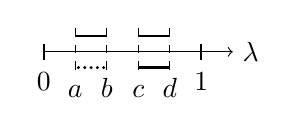
\begin{tikzpicture}[scale=2]

    % Axis
    \draw[->] (0,0) -- (1.2,0) node[right] {$\lambda$};

    % Tick marks and labels at 0 and 1
    \foreach \x/\label in {0/0, 1/1}
    {
        \draw[thick] (\x,0.05) -- (\x,-0.05);
        \node[below=4pt] at (\x,0) {$\label$};
    }

    % Two disjoint clusters
    \draw[thick] (0.2,0.1) -- (0.4,0.1);
    \draw[thick] (0.6,0.1) -- (0.8,0.1);
    % \node[above] at (0.3,0.1) {Cluster 1};
    % \node[above] at (0.7,0.1) {Cluster 2};
    % \node[left] at (0,0.1) {\small Two disjoint clusters};
    
    % Cluster with tail
    \draw[thick] (0.6,-0.1) -- (0.8,-0.1); % main cluster
    \foreach \x in {0.22,0.26,0.30,0.34,0.38} 
        \fill (\x,-0.1) circle (0.3pt); % tail eigenvalues
    % \node[below] at (0.7,-0.1) {Main cluster};
    % \node[below] at (0.3,-0.1) {Tail};
    % \node[left] at (0,-0.1) {\small Cluster with tail};
    
    % Mark points a, b, c, d
    \foreach \x/\label in {0.2/a, 0.4/b, 0.6/c, 0.8/d}
    {
        \draw[thin,dashed] (\x,0.15) -- (\x,-0.15);
        \node[above] at (\x,-0.35) {$\label$};
    }
    
\end{tikzpicture}
                    }
                \end{figure}
            }
            \only<5-8>{%
                Let $\epsilon = \frac{\|\mathbf{e}_m\|_A}{\|\mathbf{e}_0\|_A}$ relative error
                \begin{equation*}
                    1 \leq p = \min\left\{\left\lceil\frac{1}{2}\sqrt{\frac{b}{a}}\ln{\epsilon} + 1\right\rceil, N_{\text{tail}}\right\}
                \end{equation*}
            }
        \end{column}
    \end{columns}
    \only<6-8>{%
        \begin{equation*}
            \bar{m}=\left\lceil\frac{1}{2} \sqrt{\alert<7>{\frac{d}{c}}} \ln \frac{2}{\epsilon}+\left(1+\frac{1}{2} \sqrt{\alert<7>{\frac{d}{c}}} \ln \frac{4 \alert<8>{d}}{\alert<8>{e}}\right) p\right\rceil, \text{ where } e = \begin{cases}
                b, \text{ two clusters}\\
                a, \text{ cluster with tail}\\
            \end{cases}
        \end{equation*}
    }
\end{frame}

\footerinfootnotestrue
\begin{frame}[label=background,fragile]{Background: Schwarz}
    \frametitle{Background \& Literature}
    \framesubtitle{Schwarz preconditioners}
    \begin{columns}[T,onlytextwidth]
        \begin{column}{.5\textwidth}
            \begin{itemize}
                \item<1-> Derived from the Alternating Schwarz method\cite{schwarz_methods_Dolean_2015}
                \item<2-> Convergence rate depends on the overlap $\alert<2>{\delta}$ and the wave number of eigenmodes $\alert<3>{k}$
                \item<4-> As a preconditioner $M_{\text{ASM}} = \sum_{i=1}^{N_{\text{sub}}} R_i^T A_i^{-1} R_i$
                \item<5-> Need a coarse space $\alert<6>{R_0}$ to counter slowly converging modes
            \end{itemize}
        \end{column}
        \begin{column}{.49\textwidth}
            \only<1>{%
                \begin{figure}[H]
                    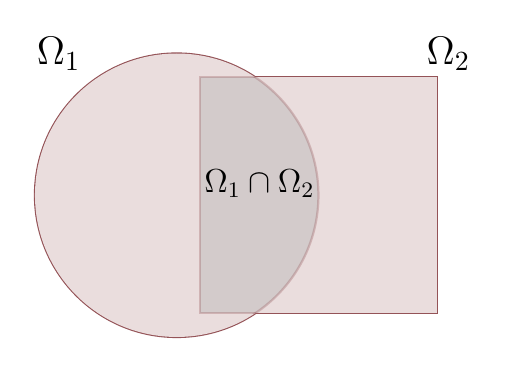
\begin{tikzpicture}[scale=1.5]
    
% Disk (left) % Smaller square (right): edges
\draw[chapter, thick] (-2,0) circle (1.2);
\draw[chapter, thick] (-1.8,-1.0) rectangle (0.2,1.0);

% Square (right) % Larger disk (left): fill
\fill[chapter!20] (-2,0) circle (1.2);
\fill[chapter!20] (-1.8,-1.0) rectangle (0.2,1.0);

% Overlapping region
\begin{scope}
  \clip (-2,0) circle (1.2);
  \fill[black!30, opacity=0.4] (-1.8,-1.0) rectangle (0.2,1.0);
\end{scope}

% Transparent edge in overlap (disk)
\begin{scope}
  \clip (-1.8,-1.0) rectangle (0.2,1.0);
  \draw[chapter, thick, opacity=0.3] (-2,0) circle (1.2);
\end{scope}

% Transparent edge in overlap (square)
\begin{scope}
  \clip (-2,0) circle (1.2);
  \draw[chapter, thick, opacity=0.3] (-1.8,-1.0) rectangle (0.2,1.0);
\end{scope}

% Labels
\node at (-3,1.2) {\Large $\Omega_1$};
\node at (0.3,1.2) {\Large $\Omega_2$};
\node at (-1.3,0.1) {\large $\Omega_1 \cap \Omega_2$};
    
\end{tikzpicture}
                    \caption{Domain decomposition with overlapping subdomains.}
                \end{figure}
            }
            \only<2-3>{%
                \begin{exampleblock}{2D Alternating Schwarz Example}
                    Let $\Omega_1 = (-\infty, \delta)\times \mathbb{R}$, $\Omega_2 = (\delta, \infty)\times \mathbb{R}$
                    \begin{align*}
                        -(\eta - \Delta) u & = f \text{ in } \mathbb{R}^2, \\
                        u                  & \text{ bounded at infinity}.
                    \end{align*}
                    Then the convergence rate is given by
                    \begin{equation*}
                        \rho_{\text{2D}}(k;\eta,\delta) = e^{-\alert<2>{\delta}\sqrt{\eta + \alert<3>k^2}}
                    \end{equation*}
                \end{exampleblock} 
            }
            \only<4-5>{%
                \begin{figure}[H]
                    \centering
                    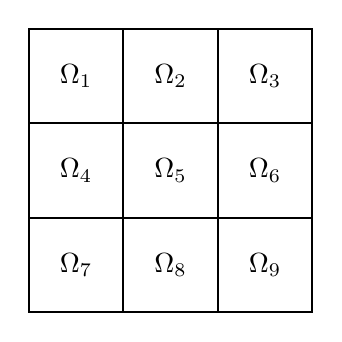
\begin{tikzpicture}[scale=1.2]

% Draw the global square domain
\draw[thick] (0,0) rectangle (3,3);
% \node at (3.3,3.3) {$\Omega$};

% Draw vertical and horizontal grid lines
\foreach \x in {1,2} {
    \draw[thick] (\x,0) -- (\x,3);
    \draw[thick] (0,\x) -- (3,\x);
}

% Label subdomains
\foreach \i in {0,1,2} {
    \foreach \j in {0,1,2} {
        \pgfmathtruncatemacro{\idx}{\i*3 + \j + 1}
        \node at (0.5 + \j, 2.5 - \i) {$\Omega_{\idx}$};
    }
}

\end{tikzpicture}
                    \caption{Domain decomposition with $N_{\text{sub}}$ subdomains.}
                \end{figure}
            }
            \only<6>{%
            \begin{block}{2-level Additive Schwarz Preconditioner}
                \begin{equation*}
                    M_{\text{ASM,2}} = \alert<6>{R_0}^T A_0^{-1} \alert<6>{R_0} + M_{\text{ASM}}
                \end{equation*}
            \end{block} 
            }
        \end{column}
    \end{columns}
\end{frame}

\footerinfootnotestrue
\begin{frame}[label=background, fragile]{Background: Coarse Spaces}
    \frametitle{Background \& Literature}
    \framesubtitle{Tailored Coarse Spaces for High-Contrast Problems}
    \only<4-6>{Figures obtained from \cite{ams_coarse_space_comp_study_Alves2024}} 
    \only<4-5>{\absimage{.73, .25}{.4}{method_legend_Alves.png}}
    \begin{columns}[T,onlytextwidth]
        \begin{column}{.5\textwidth}
            \only<1-3>{%
                \begin{itemize}
                    \item<1-> MsFEM-based: robust for high-contrast, but computationally expensive\footnote[frame]{\citeauthor{acms_coarse_space_Heinlein2018} (\citeyear{acms_coarse_space_Heinlein2018})}
                    \only<2-3>{
                        \item Generalized framework: GDSW\footnote[frame]{\citeauthor{gdsw_coarse_space_Dohrmann2008} (\citeyear{gdsw_coarse_space_Dohrmann2008})}, RGDSW\footnote[frame]{\citeauthor{rgdsw_coarse_space_Dohrmann2017} (\citeyear{rgdsw_coarse_space_Dohrmann2017})}
                    }
                        \only<3>{\item Hybrid: AMS\footnote[frame]{\citeauthor{ams_coarse_space_comp_study_Alves2024} (\citeyear{ams_coarse_space_comp_study_Alves2024})}
                    }
                \end{itemize}
            }
            \only<4>{%
                \begin{figure}[H]
                    \centering
                    \includegraphics[width=0.8\textwidth]{coefficient_function_vertex_Alves.png}
                \end{figure}
            }
            \only<5>{%
                \begin{figure}[H]
                    \centering
                    \includegraphics[width=0.8\textwidth]{coefficient_function_edges_Alves.png}
                \end{figure}
            }
        \end{column}
        \begin{column}{.5\textwidth}
            \only<2-3>{%
                \begin{figure}[H]
                    \centering
                    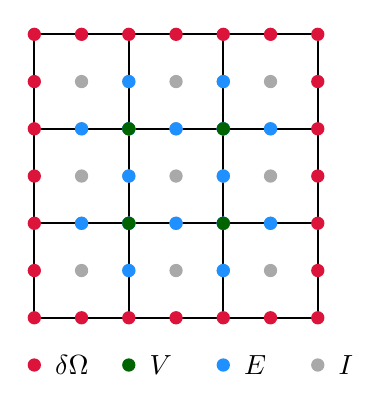
\begin{tikzpicture}[scale=1.2]

    % Colors
    \definecolor{globaledge}{RGB}{220,20,60} % crimson
    \definecolor{vertex}{RGB}{0,100,0} % dark green
    \definecolor{edge}{RGB}{30,144,255} % dodger blue
    \definecolor{interior}{RGB}{169,169,169} % dark gray
    
    % Draw the global square domain
    \draw[thick] (0,0) rectangle (3,3);
    
    % Draw vertical and horizontal grid lines
    \foreach \x in {1,2} {
        \draw[thick] (\x,0) -- (\x,3);
        \draw[thick] (0,\x) -- (3,\x);
    }
    
    % Place the 7x7 nodes
    \foreach \i in {0,...,6} {
        \foreach \j in {0,...,6} {
            % Compute position
            \pgfmathsetmacro{\x}{\i*0.5}
            \pgfmathsetmacro{\y}{\j*0.5}
    

        % Determine node type
        % Global edge (corners and boundary)
        \ifdim\x pt=0pt
            \fill[globaledge] (\x,\y) circle (2pt);
        \else\ifdim\x pt=3pt
            \fill[globaledge] (\x,\y) circle (2pt);
        \else\ifdim\y pt=0pt
            \fill[globaledge] (\x,\y) circle (2pt);
        \else\ifdim\y pt=3pt
            \fill[globaledge] (\x,\y) circle (2pt);
        \else
            % Interior node (not on boundary)
            \fill[interior] (\x,\y) circle (2pt);

            % Edge nodes (on subdomain boundaries)
            \ifdim\x pt=1pt
                \fill[edge] (\x,\y) circle (2pt);
            \else\ifdim\x pt=2pt
                \fill[edge] (\x,\y) circle (2pt);
            \fi\fi
            \ifdim\y pt=1pt
                \fill[edge] (\x,\y) circle (2pt);
            \else\ifdim\y pt=2pt
                \fill[edge] (\x,\y) circle (2pt);
            \fi\fi

            % Vertex nodes (shared by four subdomains)
            \ifdim\x pt=1pt
                \ifdim\y pt=1pt
                    \fill[vertex] (\x,\y) circle (2pt);
                \fi
                \ifdim\y pt=2pt
                    \fill[vertex] (\x,\y) circle (2pt);
                \fi
            \fi
            \ifdim\x pt=2pt
                \ifdim\y pt=1pt
                    \fill[vertex] (\x,\y) circle (2pt);
                \fi
                \ifdim\y pt=2pt
                    \fill[vertex] (\x,\y) circle (2pt);
                \fi
            \fi
        \fi\fi\fi\fi

        }
    }
    
    % Global edge
    \fill[globaledge] (0,-0.5) circle (2pt);
    \node[right=4pt] at (0,-0.5) {$\delta \Omega$};

    % Vertex
    \fill[vertex] (1,-0.5) circle (2pt);
    \node[right=4pt] at (1,-0.5) {$V$};

    % Edge
    \fill[edge] (2,-0.5) circle (2pt);
    \node[right=4pt] at (2,-0.5) {$E$};

    % Interior
    \fill[interior] (3,-0.5) circle (2pt);
    \node[right=4pt] at (3,-0.5) {$I$};

    \end{tikzpicture}
                \end{figure}
            }
            \only<4>{%
                \begin{figure}[H]
                    \centering
                    \includegraphics[width=\textwidth]{cg_iterations_coefficient_vertex_Alves.png}
                \end{figure}
            }
            \only<5>{%
                \begin{figure}[H]
                    \centering
                    \includegraphics[width=\textwidth]{cg_iterations_coefficient_edges_Alves.png}
                \end{figure}
            }
        \end{column}
    \end{columns}
    \only<6>{%
        \absimage{.5, .52}{.65}{precond_eigvals_8_and_64_subdomains_Alves.png}
    }
\end{frame}


\begin{frame}[label=results]{Structure: Results}
    \frametitle{Structure}
    \begin{itemize}
        \item Research Questions
        \item Background \& Literature
        \item {\color{tud grapefruit}Preliminary Results}
        \item Outlook
    \end{itemize}
\end{frame}

\begin{frame}[label=results]{Results: Two-cluster}
    \frametitle{Preliminary Results}
    \framesubtitle{Two-cluster case}
\end{frame}

\begin{frame}[label=results]{Results: Multi-cluster}
    \frametitle{Preliminary Results}
    \framesubtitle{Generalization to multiple clusters}
\end{frame}

\begin{frame}[label=results]{Results: Numerical Example}
    \frametitle{Preliminary Results}
    \framesubtitle{Numerical example}
\end{frame}

\begin{frame}[label=outlook]{Structure: Outlook}
    \frametitle{Structure}
    \begin{itemize}
        \item Research Questions
        \item Background \& Literature
        \item Preliminary Results
        \item {\color{tud grapefruit}Outlook}
    \end{itemize}
\end{frame}

\begin{frame}[label=outlook]{Outlook: Q1}
    \frametitle{Outlook}
    \framesubtitle{Research Question 1 answered}
\end{frame}

\begin{frame}[label=outlook]{Outlook: Q3}
    \frametitle{Outlook}
    \framesubtitle{Research question 3 answered}
\end{frame}

\begin{frame}[label=outlook]{Outlook: Next steps}
    \frametitle{Outlook}
    \framesubtitle{Next steps}
    \begin{itemize}
        \item Work on answering research questions 4, 5, and 6.
    \end{itemize}
\end{frame}

\begin{frame}[label=outlook]{Outlook: Open Challenge}
    \frametitle{Outlook}
    \framesubtitle{Open Challenge}
    \begin{itemize}
        \item How to answer research question 2?
    \end{itemize}
\end{frame}

\end{document}